\documentclass{article}
\usepackage{amsmath,natbib,fullpage,caption,graphicx,lineno}
\title{Statistical chronometry of meteorites revisited}
\author{Pieter Vermeesch\\\emph{University College London, UK}\\
  and\\
Steven J. Desch\\\emph{Arizona State University, USA}}
\begin{document}
\linenumbers
\maketitle

\begin{abstract}
  The chronology of the early solar system rests on extinct
  (\textsuperscript{26}Al/\textsuperscript{26}Mg,
  \textsuperscript{53}Mn/\textsuperscript{53}Cr,
  \textsuperscript{182}Hf/\textsuperscript{182}W) and extant
  (\textsuperscript{207}Pb/\textsuperscript{206}Pb) chronometers,
  which should agree for rapidly cooled meteorites from isotopically
  homogeneous parts of the solar system. Testing this concordance
  requires a statistical framework. Here we introduce two approaches
  to statistical chronometry of meteorites.  In a first approach, we
  revisit the weighted-mean based approach of Desch et al. (2023,
  doi:10.1016/j.icarus.2023.115607 and
  doi:10.1016/j.icarus.2023.115611), which tracks events forward in
  time from the start of the solar system, $t_{\mathit{SS}}$.  After
  fixing an error in the model's original formulation, we show that
  its application to a previously published compilation of 38
  multi-dated meteorite dates reveals statistically significant
  overdispersion with respect to the analytical uncertainties.  A
  second approach is to build the statistical chronology counting
  backward in time, starting from the present and converting
  extinct-nuclide dates to `Pb--Pb time' through a single offset
  parameter estimated by weighted regression with a fixed unit
  slope. Applying the second algorithm to the 38-sample data
  compilation yields the same conclusion of statistically significant
  overdispersion. Extending the regression to a random-effects model
  allows the excess dispersion to be quantified. It is equivalent to
  up to 10\% heterogeneity in initial
  \textsuperscript{26}Al/\textsuperscript{27}Al,
  \textsuperscript{53}Mn/\textsuperscript{55}Mn or
  \textsuperscript{182}Hf/\textsuperscript{180}Hf, or 100--800\,kyr of
  excess scatter in Pb--Pb dates.  Whether the cause of the excess
  dispersion is astrophysical or analytical remains
  unresolved. Routine measurement of
  \textsuperscript{238}U/\textsuperscript{235}U in Pb--Pb dated
  mineral phases and more realistic statistical models for isochron
  selection may help to separate these causes.
\end{abstract}

\section{Introduction}
\label{sec:intro}

The chronology of the early solar system can be constrained from the
radiogenic decay products of extinct (\textsuperscript{26}Al,
\textsuperscript{53}Mn, \textsuperscript{182}Hf) and extant
(\textsuperscript{235}U, \textsuperscript{238}U) nuclides in
meteorites. The extinct nuclides form the basis of relative
chronometers, which can be used to estimate the age difference between
pairs of meteorites. In principle, the extant nuclides can be used to
anchor meteorites in absolute time, counting back from the present.
However, in practice the precision of such absolute dates is limited
by the analytical uncertainty of the decay constants
\citep{ludwig2000}. For the
\textsuperscript{207}Pb/\textsuperscript{206}Pb method, this
uncertainty amounts to ca.~9\,Myr ($2\,\sigma$) at 4567\,Ma
(Figure~\ref{fig:lambda_err}). The decay constant uncertainty is
greatly reduced when calculating the difference between two similar
\textsuperscript{207}Pb/\textsuperscript{206}Pb dates
(Figure~\ref{fig:lambda_err}). For example, a 10\,Myr age difference
near the onset of the solar system is associated with a decay constant
uncertainty of only 7\,kyr.  Therefore, when comparing
\textsuperscript{207}Pb/\textsuperscript{206}Pb dates within the
4550-4568\,Ma age range, decay constant uncertainties can be safely
ignored, turning the
\textsuperscript{207}Pb/\textsuperscript{206}Pb-method into a relative
chronometer with similar precision as the extinct
chronometers.\medskip

\noindent\begin{minipage}{.4\linewidth}
  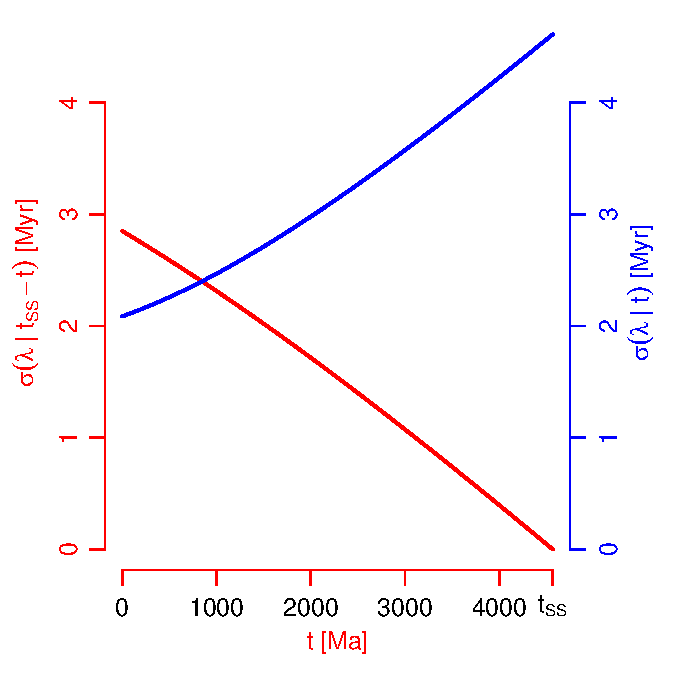
\includegraphics[width=\linewidth]{lambda_err.pdf}
\end{minipage}
\begin{minipage}{.6\linewidth}
\captionof{figure}{Decay constant uncertainty as a function of the
  \textsuperscript{207}Pb/\textsuperscript{206}Pb age $t$ (blue); and
  the age difference between a meteorite of age $t$ and the start of
  the solar system $t_{\mathit{SS}}$ (red).}
\label{fig:lambda_err}
\end{minipage}

For rapidly cooled meteorites in isotopically homogenised regions of
the early solar system, extinct and extant chronometers should be
concordant. Jointly considering a basket of such double-dated
meteorites leads to the establishment of a `statistical chronology' of
those meteorites. This paper presents two approaches to this
problem. A first approach is to establish a chronology for the early
solar system counting forward in time from the start of the solar
system, $t_{\mathit{SS}}$, using the scatter of double-, triple- and
quadruple-dated meteorites around their weighted means
(Section~\ref{sec:means}).  A second approach is to build the
statistical chronology counting backward in time, starting from the
present and using linear regression instead of weighted means
(Section~\ref{sec:regression}).\medskip

Section~\ref{sec:application} applies both approaches to a collection
of 11 rapidly cooled meteorites compiled by
\citet{desch2023a,desch2023b}. Previous statistical analysis of this
database using the first approach suggested concordance of the
Al--Mg, Mn--Cr, Hf--W and Pb--Pb methods. After
fixing an error in \citet{desch2023a,desch2023b}'s calculations,
we come to a different conclusion and find a small but statistically
significant amount of excess dispersion in the data.
Section~\ref{sec:discussion} quantifies this overdispersion
by modifying the linear regression method.\medskip

This paper will use the following definitions:

\begin{description}
\item{$t_{\mathit{SS}}:$} the start of the solar system, measured from the present;
\item{$t_{\mathit{Al}}$, $t_{\mathit{Pb}}$, $t_{\mathit{Mn}}$, $t_{\mathit{Hf}}$:} the Al--Mg, Pb--Pb,
  Mn--Cr and Hf--Cr date, respectively, measured from the present;
\item{$\Delta t_{\ast}$} $= t_{\mathit{SS}} - t_{\ast}$, where $\ast
  \in \{\mathit{Al}, \mathit{Pb}, \mathit{Mn}, \mathit{Hf}\}$;
\item{$\lambda_{26}$, $\lambda_{53}$:} the decay constant of
  \textsuperscript{26}Al and \textsuperscript{53}Mn, respectively;
\item{$\left[{}^{y}\mbox{X}/^{x}\mbox{X}\right]_{\mathit{SS}}$:} the
  ${}^{y}\mbox{X}/^{x}\mbox{X}$ (e.g.,
  ${}^{27}\mbox{Al}/^{26}\mbox{Al}$)-ratio of the solar system at
  $t_{\mathit{SS}}$;
\item{$\left[{}^{y}\mbox{X}/^{x}\mbox{X}\right]_{0}$:} the initial
  ${}^{y}\mbox{X}/^{x}\mbox{X}$-ratio of a meteorite at the time
  of its formation;
\item{$\sigma[\ast]$:} the analytical uncertainty (estimated standard
  deviation) of $\ast$;
\item{$\chi^2$:} the chi-square statistic for homogeneity;
\item{$\nu$:} the number of degrees of freedom of the chi-square test;
\item{MSWD:} the mean square weighted deviation, defined as MSWD =
  $\chi^2/\nu$.
\end{description}

\section{Approach 1: $t_{\mathit{SS}} \rightarrow t$}
\label{sec:means}

\citet{desch2023a} define $t_{\mathit{SS}}$ as the time when the
\textsuperscript{26}Al/\textsuperscript{27}Al-ratio of the Solar
System was
$({}^{26}\mbox{Al}/{}^{27}\mbox{Al})_{\mathit{SS}}={5.23}\times{10}^{-5}$,
assuming isotopic homogeneity. The actual value of $t_{\mathit{SS}}$ is then
estimated by minimising the sum of the squared differences between
$\Delta{t}_{Al} = \dfrac{1}{\lambda_{26}} \left(
\ln\left[\dfrac{{}^{26}\mbox{Al}}{{}^{27}\mbox{Al}}\right]_{\mathit{SS}} -
\ln\left[\dfrac{{}^{26}\mbox{Al}}{{}^{27}\mbox{Al}}\right]_{0} \right)
$ and $\Delta{t}_{Pb} = t_{\mathit{SS}} - t_{Pb}$ for a `basket' of
double-dated meteorites that are thought to have achieved simultaneous
isotopic closure for both systems. Given a set of $n$ double-dated
meteorites, \citet{desch2023a} test the concordance of the Al--Mg and
Pb--Pb dates by find the value of $t_{\mathit{SS}}$ that minimises the
chi-square statistic:
\begin{equation}
  \chi^2 = \sum\limits_{i=1}^{n}\sum\limits_{\ast\in\{Al,Pb\}}
  \left(\dfrac{\Delta t_{\ast,i}-\Delta\bar{t}_i}{\sigma\left[t_{\ast,i}\right]}\right)^2
  \label{eq:chi2}
\end{equation}

\noindent where $\bar{t}_i$ is the error-weighted mean of the Al--Mg
and Pb--Pb dates of the $i$\textsuperscript{th} meteorite. If all $n$
meteorites are concordant, and if analytical uncertainty is the only
source of dispersion, then $\chi^2$ is expected to follow a chi-square
distribution with $\nu$ degrees of freedom. This expectation can be
used to formally test the concordance of the data: $\chi^2$-values
indicate homogeneity, high values ($\gg\nu$) indicate overdispersion.
\citet{desch2023a} posit that $\nu = 2\,n-1$, assuming that
$\Delta{t}_{Al,i}$ and $\Delta{t}_{Pb,i}$ are statistically
independent. This is wrong. In reality, $\Delta{t}_{Al,i}$ and
$\Delta{t}_{Pb,i}$ are perfectly anti-correlated, so that the correct
number of degrees of freedom is $\nu = n-1$. This value accounts for
the fact that $\chi^2$ comprises $n$ weighted means of paired values
(each of which represents one degree of freedom) minus one degree of
freedom because $t_{\mathit{SS}}$ is estimated from the data.\medskip

Equation~\ref{eq:chi2} can be generalised to more than two
chronometers.  Suppose that the collection of $n$ meteorites comprises
of $n_2$ double-dated, $n_3$ triple-dated and $n_4$ quadruple-dated
meteorites, then \citet{desch2023b} posit that $\nu = 2\,n_2 + 3\,n_3
+ 4\,n_4 - m$, where $m$ is the number of nuisance parameters to be
estimated as part of the optimisation among $t_{\mathit{SS}}$,
$\left[^{53}\mbox{Mn}/^{55}\mbox{Mn}\right]_{\mathit{SS}}$,
$\left[^{182}\mbox{Hf}/^{180}\mbox{Hf}\right]_{\mathit{SS}}$ and
$\lambda_{53}$. This is also wrong, with the correct value being $\nu
= n_2 + 2\,n_3 + 3\,n_4 - m$. This value accounts for the fact that
the weighted mean of $N$ values has $N-1$ degrees of freedom, so that
the sum of the $\chi^2$-values for $n_N$ weighted means has $(N-1)
\,n_N$ degrees of freedom.

\section{Approach 2: $t \leftarrow \mbox{present}$}
\label{sec:regression}

Approach~1 defines $t_{\mathit{SS}}$ in terms of an assumed value for
$({}^{26}\mbox{Al}/{}^{27}\mbox{Al})_{\mathit{SS}}$, and using a basket of
double-dated meteorites.  Future updates to the basket would result in
new estimates for $t_{\mathit{SS}}$. However, this is not the only option. A
mathematically equivalent use of the basket would be to fix $t_{\mathit{SS}}$
and treat $({}^{26}\mbox{Al}/{}^{27}\mbox{Al})_{\mathit{SS}}$ as an unknown. In
fact, the choice of $t_{\mathit{SS}}$ is completely arbitrary and can be
avoided altogether by expressing the Al/Mg-dates in `Pb/Pb-time', by
counting time from the present instead of from $t_{\mathit{SS}}$. This can be
done by finding the offset $A$ that minimises the misfit between
$t_{Al}$ and $t_{Pb}$, where
\begin{equation}
  t_{Al} = A +
  \frac{1}{\lambda_{26}}\ln\left(\frac{{}^{26}\mbox{Al}}{{}^{27}\mbox{Al}}\right)_{0}
  \label{eq:A}
\end{equation}

\noindent in which $A = t_{\mathit{SS}} -
\ln\left({}^{26}\mbox{Al}/{}^{27}\mbox{Al}\right)_{\mathit{SS}}/\lambda_{26}$.
Any change to the basket of double-dated meteorites would change $A$
and, hence, $t_{Al}$. However, $t_{Pb}$ would remain unaffected,
unlike \citet{desch2023a}'s $\Delta{t}_{Pb}$ and $\Delta{t}_{Al}$,
which would both change.\medskip

The offset parameter $A$ can be estimated by weighted least squares
regression with a fixed unit slope \citep{vermeesch2024}. The
dispersion of the data around the 1:1 line is quantified by a
chi-square statistic with $n-1$ degrees of freedom, i.e. exactly as
under Approach~1. Mn--Cr and Hf--W data can be treated in the same
way.

\section{Application to the \citet{desch2023b} database}
\label{sec:application}

\citet{desch2023a,desch2023b} applied Approach~1 to the compilation of
meteorites shown in Table~\ref{tab:desch}. In their detailed survey of
the literature, they adjusted the published results of several studies
in different three ways. First, they recalculated the Pb--Pb dates of
some meteorites by retrospectively adjusting the
${}^{238}\mbox{U}/{}^{235}\mbox{U}$-ratios by 0.3\textperthousand to
account for possible U-fractionation between pyroxene and whole rock
\citep{tissot2017}. Second, they recalculated the Pb--Pb isochrons for
certain meteorites using a different selection of aliquots than
reported in the original publications. Third, they treated the
\textsuperscript{53}Mn-decay constant as an unknown and optimised the
$\lambda_{53}$-value that brought the Mn--Cr data as close as possible
to concordance with the other chronometers. \medskip

Applying Equation~\ref{eq:chi2} to the corrected data of
Table~\ref{tab:desch}, \citet{desch2023b} report a $\chi^2$-value of
47.94 for the 38 meteorite dates, assuming $\nu=37-4=34$ degrees of
freedom. Under this assumption, the p-value for the chi-square test is
0.057, which is greater than 0.05 and failure to reject the null
hypothesis that the meteorite ages are all concordant. However, as
discussed in Section~\ref{sec:means}, the correct number of degrees of
freedom is not $34$ but
$\nu={6}\times{1}+{6}\times{2}+{2}\times{3}-4=20$. Using this correct
value yields a p-value of 0.00043, resulting in a rejection of the
null hypothesis.\medskip

\citet{desch2023b} also present a second $\chi^2$-value of 35.97 with
$\nu=33$ degrees of freedom by removing the Mn--Cr date of NWA~4801.
This results in a p-value of 0.33, which is again seemingly compatible
with the basket of meteorites achieving concordant isotopic closure
for all four isotopic systems. However, combining the same statistic
with the correct number of degrees of freedom ($\nu=19$) produces a
p-value of 0.011, which contradicts this conclusion.

\captionof{table}{Summary table for the database of
  \citet{desch2023b}. Headers use the following shorthand notation:
  $\mathit{Al}_0 \equiv
  \left(^{26}\mbox{Al}/^{27}\mbox{Al}\right)_0$, $\mathit{Mn}_0
  \equiv \left(^{53}\mbox{Mn}/^{55}\mbox{Mn}\right)_0$,
  $\mathit{Hf}_0 \equiv
  \left(^{182}\mbox{Hf}/^{180}\mbox{Hf}\right)_0$;
  $t_{\mathit{orig}}$ stands for the original Pb--Pb dates extracted
  from the literature; $t_{\mathit{adj}}$ represents the adjusted
  values used by \citet{desch2023b}.}
\label{tab:desch}
\begin{tabular}{@{}r@{~}|@{~}c@{~}c@{~}c@{~}c@{~}c@{~}c@{~}|@{~}c@{~}c@{~}c@{~}c@{}}
  sample & $\mathit{Al}_0$ & $2\sigma(\mathit{Al}_0)$ &
  $\mathit{Mn}_0$ & $2\sigma(\mathit{Mn}_0)$ &
  $\mathit{Hf}_0$ & $2\sigma(\mathit{Hf}_0)$ &
  $t_{\mbox{orig}}$ & $2\sigma\left(t_{\mathit{orig}}\right)$ &
  $t_{\mbox{adj}}$ & $2\sigma\left(t_{\mathit{adj}}\right)$ \\ \hline
  D'Orbigny & 3.93 &  0.39 & 3.23 & 0.03 & 7.15 & 0.17 & 4564.42 & 0.12 & 4563.24 & 0.21 \\
  SAH 99555 & 3.64 & 0.18 & 3.28 & 0.17 & 6.87 & 0.15 & 4564.614 & 0.131 & 4563.51 & 0.24 \\
  NWA 1670 & 5.92 & 0.59 & 2.85 & 0.92 & & & 4565.39 & 0.24 & 4564.02 & 0.66 \\
  NWA 1296 & & & & & 7.01 & 0.28 & 4564.2 & 0.45 & 4563.02 & 0.45 \\
  LEW 86010 & & & 1.35 & 0.05 & 4.8 & 0.42 & 4558.55 & 0.15 & & \\
  NWA 4590 & & & 0.85 & 0.4 & 4.63 & 0.17 & 4557.76 & 0.38 & 4557.57 & 0.38 \\
  NWA 4801 & & & 0.96 & 0.04 & 4.52 & 0.16 & 4556.91 & 0.21 & 4556.63 & 0.28 \\
  Angra do Reis & & & 1.1 & 0.4 & 4.02 & 0.24 & 4556.45 & 0.29 & 4556.26 & 0.29 \\
  NWA 2999 & & & & & 5.43 & 0.34 & 4560.74 & 0.47 & 4560.55 & 0.47 \\
  Asuka 881394 & 13.07 & 0.56 & 3.86 & 0.23 & & & 4564.95 & 0.53 & 4564.76 & 0.53 \\
  Ibitira & & & 1.06 & 0.5 & & & 4556.75 & 0.57 & 4556.56 & 0.57 \\
  NWA 7325 & 3.03 & 0.14 & & & & & 4563.9 & 1.7 & 4563.7 & 1.7 \\
  NWA 2976 & 4.05 & 0.15 & & & & & 4563.16 & 0.57 & 4563.16 & 0.57 \\
  NWA 6704 & 3.15 & 0.38 & 2.59 & 0.34 & & & 4562.76 & 0.26 & 4562.76 & 0.26\\
\end{tabular}\medskip

We now proceed to subject Table~\ref{tab:desch} to
Approach~2. Figure~\ref{fig:regression_original} compares the original
Pb--Pb dates with the Al--Mg, Mn--Cr and Hf--W dates,
respectively. For each of the three pairs of measurements, the offset
$A$ was found by minimising the weighted sum of the square residuals
around the 1:1 line, using the algorithm of \citet{vermeesch2024}. All
three cases exhibit high MSWD-values and fail the chi-squared test for
homogeneity. This indicates that the data are overdispersed with
respect to the analytical uncertainties.\medskip

The excess dispersion of the data around the 1:1 line in
Figure~\ref{fig:regression_original} can be attributed to either (i)
$({}^{26}\mbox{Al}/{}^{27}\mbox{Al})_{\mathit{SS}}$-heterogeneity
\citep{krestianinov2023}; (ii) partial resetting of the
${}^{207}\mbox{Pb}/{}^{206}\mbox{Pb}$-clock during transient heating
events \citep{desch2023a}; (iii)
${}^{238}\mbox{U}/{}^{235}\mbox{U}$-fractionation \citep{tissot2017};
or (iv) inappropriate outlier rejection prior to regression of the
${}^{26}\mbox{Mg}/{}^{27}\mbox{Mg}$ and/or
${}^{207}\mbox{Pb}/{}^{206}\mbox{Pb}$ data
\citep{desch2023a,vermeesch2026f}.\medskip

\citet{desch2023a,desch2023b} adjusted the Pb--Pb dates in
Table~\ref{tab:desch} to remove factors (ii) and (iii).  This
adjustment does indeed lowers the MSWD-value considerably
(Figure~\ref{fig:regression_adjusted}).  Nevertheless, the three
pairwise comparisons still fail the chi-square test. This either means
that the dispersion is caused by scenario (i), or that the adjustment
has not gone far enough. In any case, Approach~2 leads to the same
conclusion as Approach~1, namely that the different chronometers are
not concordant.\medskip

Section~\ref{sec:discussion} will extend Approach~2 to treat the
various sources of heterogeneity as an unknown, whose effect can be
estimated from the data.

\noindent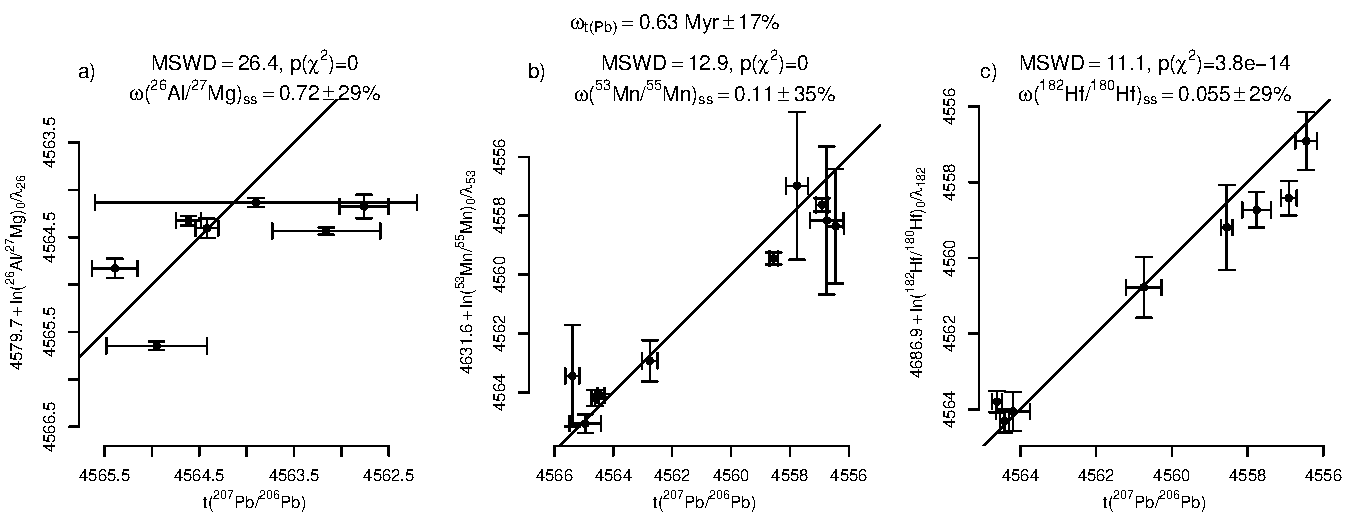
\includegraphics[width=\linewidth]{Desch2_original.pdf}
\captionof{figure}{Pairwise comparison of the original Pb--Pb dates of
  Table~\ref{tab:desch} with Al--Mg (panel~a), Mn--Cr (panel~b) and
  Hf--W (panel~c) dates for the same, rapidly cooled meteorites. The
  1:1 lines were obtained using the optimal $A$-values
  (Equation~\ref{eq:A}). All three datasets are overdispersed around
  this line with respect to the analytical uncertainties
  (MSWD$\,\gg\,1$). $\omega$-values are the estimated standard
  deviations of the excess dispersion, assuming normality
  (Section~\ref{sec:discussion}). This dispersion can either be
  attributed to the Pb--Pb data, or to the initial
  $({}^{26}\mbox{Al}/{}^{27}\mbox{Al})_{\mathit{SS}}$,
  $({}^{53}\mbox{Mn}/{}^{55}\mbox{Mn})_{\mathit{SS}}$ or
  $({}^{182}\mbox{Hf}/{}^{180}\mbox{Hf})_{\mathit{SS}}$-values. Uncertainties
  are reported as standard errors.}
\label{fig:regression_original}

\section{Quantifying dispersion}
\label{sec:discussion}

\noindent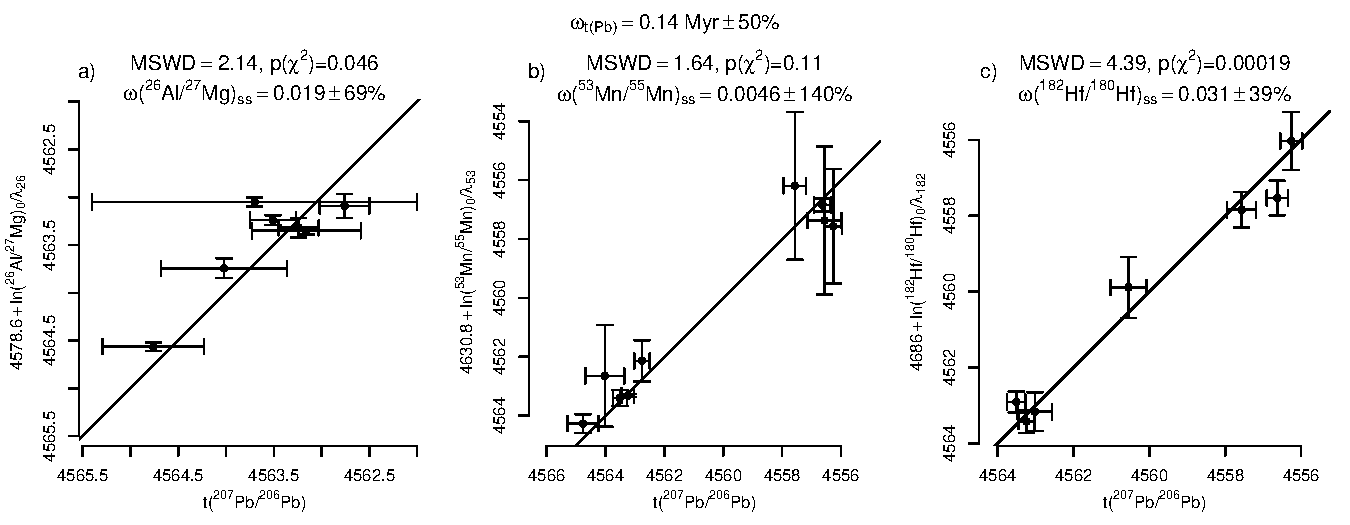
\includegraphics[width=\linewidth]{Desch2_adjusted.pdf}
\captionof{figure}{Similar to Figure~\ref{fig:regression_original},
  but using the adjusted Pb--Pb dates of
  Table~\ref{tab:desch}.\medskip}
\label{fig:regression_adjusted}

The observed overdispersion can be mathematically captured by random
effects models that attribute the excess dispersion to either the x-
or the y-variables of Figure~\ref{fig:regression_original}. The
problem can be formalised by introducing the following definitions:
\begin{description}
  \item{$t_x(m,i)$:} the measured Pb--Pb date of the
    $i$\textsuperscript{th} aliquot;
  \item{$t_y(m,i)$:} the measured Al--Mg, Mn--Cr or W--Hf date of the
    $i$\textsuperscript{th} aliquot;
  \item{$\delta_x(i)$ and $\delta_y(i)$:} the offset between the true
    x- and y-value caused by dispersion of the true Pb--Pb age, or by
    the heterogeneity of $({}^{26}\mbox{Al}/{}^{27}\mbox{Al})_{\mathit{SS}}$,
    $({}^{53}\mbox{Mn}/{}^{55}\mbox{Mn})_{\mathit{SS}}$ or
    $({}^{182}\mbox{Hf}/{}^{180}\mbox{Hf})_{\mathit{SS}}$, respectively;
  \item{$x(i) (+ \delta_x(i))$:} the true Pb--Pb age of the
    $i$\textsuperscript{th} aliquot;
  \item{$y(i) (+ \delta_y(i))$:} the true Al--Mg, Mn--Cr or Hf--W age
    of the $i$\textsuperscript{th} aliquot;
  \item{$\epsilon_x(i), \epsilon_y(i)$:} residuals, caused by
    analytical uncertainty.
\end{description}

Using these definitions, two random effects models can be formulated:
\begin{equation}
  \mbox{Model~3x:~}
  \begin{cases}
    t_{x}(m,i) = x(i) + \delta_x(i) + \epsilon_x(i) \\
    t_{y}(m,i) = x(i) + \epsilon_y(i)
  \end{cases}
  \mbox{,~Model~3y:}
  \begin{cases}
    t_{x}(m,i) = y(i) + \epsilon_x(i) \\
    t_{y}(m,i) = y(i) + \delta_y(i) + \epsilon_y(i)
  \end{cases}
  \label{eq:model3xy}
\end{equation}

To keep the problem tractable, it is necessary to make the simplifying
assumption that $\delta_x(i)$, $\delta_y(i)$, $\epsilon_x(i)$ and
$\epsilon_y(i)$ were drawn from normal distributions with zero mean.
For $\epsilon_x(i)$ and $\epsilon_y(i)$, this assumption is
reasonable. For $\delta_x(i)$ and $\delta_y(i)$, that is not
necessarily so. For example, it is possible that there were multiple
reservoirs with distinctly different
$({}^{26}\mbox{Al}/{}^{27}\mbox{Al})_{\mathit{SS}}$-values. However,
Figure~\ref{fig:regression_adjusted}a) only contains 7 double-dates,
which is too small to identify such multi-modality. Therefore, the
simple normal assumption is necessary. The model can easily be
modified to capture more realistic scenarios should a sufficiently
large database of multi-dated meteorites become available in the
future.\medskip

For model~3x, we will assume that the $\delta_x(i)$-values were drawn
from a normal distribution with zero mean and standard deviation
$\omega_{\mathit{t(Pb)}}$ (units: Myr). For model~3y, we will assume
that the $\delta_y(i)$-values were drawn from a normal distribution
with zero mean and standard deviation $\omega_y\lambda_y$ (units:
none), which captures the dispersion of the
$({}^{26}\mbox{Al}/{}^{27}\mbox{Al})_{\mathit{SS}}$,
$({}^{53}\mbox{Mn}/{}^{55}\mbox{Mn})_{\mathit{SS}}$ or
$({}^{182}\mbox{Hf}/{}^{180}\mbox{Hf})_{\mathit{SS}}$-values,
depending on the dataset used to solve the problem. Note that model~3x
can be solved using the combined dataset of Al--Mg, Mn--Cr and Hf--W
measurements.\medskip

The analysis shows that the overdispersion of the adjusted meteorite
dataset can either be explained by:
\begin{enumerate}
\item 0.5--7.5\% heterogeneity of the
  $({}^{26}\mbox{Al}/{}^{27}\mbox{Al})_{\mathit{SS}}$-ratio (at $2\sigma$,
  i.e. $\exp[\ln(0.019)\pm{2\times0.69}]$;
  Figure~\ref{fig:regression_adjusted}a).
\item 2--7.5\% heterogeneity of the 
  $({}^{53}\mbox{Mn}/{}^{55}\mbox{Mn})_{\mathit{SS}}$-ratio;
\item 1.4--6.8\% heterogeneity of the
  $({}^{182}\mbox{Hf}/{}^{180}\mbox{Hf})_{\mathit{SS}}$-ratio;
\end{enumerate}

or by

\begin{enumerate}
  \setcounter{enumi}{3}
\item 100--800\,ka excess dispersion in the Pb--Pb isochron data,
  caused by partial resetting during transient heating events
  \citep{desch2023a} or by possible over-zealous outlier rejection,
  which unduly promotes precision over accuracy
  \citep{vermeesch2026f}.
\end{enumerate}

\section{Conclusion}
\label{sec:conclusion}

This paper presented two equivalent approaches to statistical
chronometry, using an existing compilation of multi-dated meteorites
originally presented by \citet{desch2023a}. The first approach counts
time forward in time, from $t_{\mathit{SS}}$, which is treated as an
unknown parameter, and is estimated assuming an assumed
$\left(^{26}\mbox{Al}/^{27}\mbox{Al}\right)_{\mathit{SS}}$-value of
$5.23\times{10}^{-5}$ along with
$\left(^{53}\mbox{Mn}/^{55}\mbox{Mn}\right)_{\mathit{SS}}$,
$\left(^{182}\mbox{Hf}/^{180}\mbox{Hf}\right)_{\mathit{SS}}$ and
(optionally) $\lambda_{53}$. Using the correct number of degrees of
freedom, this approach reveals statistically significant dispersion
between the extinct and extant chronometers. The second approach uses
bivariate linear regression of double-dated meteorites to assess the
concordance of the meteorite database. It does not treat
$t_{\mathit{SS}}$,
$\left(^{53}\mbox{Mn}/^{55}\mbox{Mn}\right)_{\mathit{SS}}$ and
$\left(^{182}\mbox{Hf}/^{180}\mbox{Hf}\right)_{\mathit{SS}}$ as
explict unknowns, but instead converts the
$\ln\left(^{26}\mbox{Al}/^{27}\mbox{Al}\right)_0$
$\ln\left(^{53}\mbox{Mn}/^{55}\mbox{Mn}\right)_0$
$\ln\left(^{182}\mbox{Hf}/^{180}\mbox{Hf}\right)_0$ logratios to
absolute ages using a linear transformation
(Equation~\ref{eq:A}). Applying the second approach to the
\citet{desch2023a} leads to the same conclusion as the first approach,
exhibiting statistically significant dispersion of the extinct and the
extant chronometers.\medskip

The regression approach marks a step forward in the development of a
statistical chronometry for meteorites, by going from a simple test
for statistical homogeneity, to the quantification of heterogeneity.
This is important because, to paraphrase statistician George Box ``all
hypotheses are wrong (in some decimal place)''. Given a sufficiently
large or precise database of multi-dated meteorites, even the smallest
degree of heterogeneity eventually becomes detectable. The chi-square
test cannot determine whether this heterogeneity has an astrophysical
or analytical cause. Likely, a combination of both factors is at
play. In order to disentangle the relative contributions of these two
possibilities, improved analytical and statistical approaches are
needed.\medskip

Analytical improvements include the addition of
\textsuperscript{238}U/\textsuperscript{235}U measurements in the same
mineral phase as the Pb-isotope measurements. Although this is
challenging to do in small (or U-poor) samples, it removes the need
for the nominal 0.3\textperthousand correction applied by
\citet{desch2023a,desch2023b} to many of the meteorites in
Table~\ref{tab:desch}. Statistical improvements include a more
rigorous selection of aliquots to include in Pb--Pb isochrons.  For
example, \citet{desch2023a} present a detailed discussion of
\citet{schiller2015}'s Pb--Pb dataset for NWA~1670 and show that there
are at least three statistically equivalent ways to form an isochron
through these data, with significantly different ages. To solve this
problem, it would be useful to abandon the binary notion that aliquots
fell either `on' or `off' the concordia line. A statistically more
rigorous approach would be to assign a finite probability to each
category for each aliquot, similar to the random effects model of
Section~\ref{sec:discussion}. Such a `leftmost isochron' algorithm was
recently implemented in \texttt{IsoplotR} \citep{vermeesch2018c} and
will be discussed in a forthcoming publication.

\section*{Acknowledgments}

This research has been supported by the Natural Environment Research
Council (grant no. NE/T001518/1), awarded to PV.

\begin{thebibliography}{9}
\providecommand{\natexlab}[1]{#1}
\providecommand{\url}[1]{\texttt{#1}}
\expandafter\ifx\csname urlstyle\endcsname\relax
  \providecommand{\doi}[1]{doi: #1}\else
  \providecommand{\doi}{doi: \begingroup \urlstyle{rm}\Url}\fi

\bibitem[Desch et~al.(2023{\natexlab{a}})Desch, Dunlap, Dunham, Williams, and
  Mane]{desch2023a}
Desch, S.~J., Dunlap, D.~R., Dunham, E.~T., Williams, C.~D., and Mane, P.
\newblock {Statistical chronometry of meteorites. I. A Test of $^{26}$Al
  homogeneity and the Pb-Pb age of the solar system's $t=0$}.
\newblock \emph{Icarus}, 402:\penalty0 115607, 2023{\natexlab{a}}.

\bibitem[Desch et~al.(2023{\natexlab{b}})Desch, Dunlap, Williams, Mane, and
  Dunham]{desch2023b}
Desch, S.~J., Dunlap, D.~R., Williams, C.~D., Mane, P., and Dunham, E.~T.
\newblock {Statistical chronometry of Meteorites: II. Initial abundances and
  homogeneity of short-lived radionuclides}.
\newblock \emph{Icarus}, 402:\penalty0 115611, 2023{\natexlab{b}}.

\bibitem[Krestianinov et~al.(2023)Krestianinov, Amelin, Yin, Cary, Huyskens,
  Miller, Dey, Hibiya, Tang, Young, et~al.]{krestianinov2023}
Krestianinov, E., Amelin, Y., Yin, Q.-Z., Cary, P., Huyskens, M.~H., Miller,
  A., Dey, S., Hibiya, Y., Tang, H., Young, E.~D., et~al.
\newblock {Igneous meteorites suggest Aluminium-26 heterogeneity in the early
  Solar Nebula}.
\newblock \emph{Nature Communications}, 14\penalty0 (1):\penalty0 4940, 2023.

\bibitem[Ludwig(2000)]{ludwig2000}
Ludwig, K.~R.
\newblock {Decay constant errors in U--Pb concordia-intercept ages}.
\newblock \emph{Chemical Geology}, 166\penalty0 (3):\penalty0 315--318, 2000.

\bibitem[Schiller et~al.(2015)Schiller, Connelly, Glad, Mikouchi, and
  Bizzarro]{schiller2015}
Schiller, M., Connelly, J.~N., Glad, A.~C., Mikouchi, T., and Bizzarro, M.
\newblock {Early accretion of protoplanets inferred from a reduced inner solar
  system ${}^{26}$Al inventory}.
\newblock \emph{Earth and Planetary Science Letters}, 420:\penalty0 45--54,
  2015.

\bibitem[Tissot et~al.(2017)Tissot, Dauphas, and Grove]{tissot2017}
Tissot, F.~L., Dauphas, N., and Grove, T.~L.
\newblock {Distinct $^{238}$U/$^{235}$U ratios and REE patterns in plutonic and
  volcanic angrites: Geochronologic implications and evidence for U isotope
  fractionation during magmatic processes}.
\newblock \emph{Geochimica et Cosmochimica Acta}, 213:\penalty0 593--617, 2017.

\bibitem[Vermeesch(2018)]{vermeesch2018c}
Vermeesch, P.
\newblock {\texttt{IsoplotR}: a free and open toolbox for geochronology}.
\newblock \emph{Geoscience Frontiers}, 9:\penalty0 1479--1493, 2018.
\newblock \doi{10.1016/j.gsf.2018.04.001}.

\bibitem[Vermeesch(2026)]{vermeesch2026f}
Vermeesch, P.
\newblock Too good to be true: Underdispersion in geochronology.
\newblock \emph{EGUsphere}, 2026:\penalty0 1--26, 2026.
\newblock \doi{10.5194/egusphere-2026-2783}.

\bibitem[Vermeesch(2024)]{vermeesch2024}
Vermeesch, P.
\newblock {Errorchrons and anchored isochrons in IsoplotR}.
\newblock \emph{Geochronology}, 6\penalty0 (3):\penalty0 397--407, 2024.

\end{thebibliography}

%\bibliographystyle{/home/pvermees/Dropbox/abbrvplainnat.bst}
%\bibliography{/home/pvermees/Dropbox/biblio.bib}

\end{document}
